\documentclass{article} % For LaTeX2e
\usepackage{nips_adapted,times}
\usepackage{hyperref}
\usepackage{url}
\usepackage{listings}
\usepackage{xcolor}
\usepackage{graphicx}
\definecolor{codeblue}{rgb}{0.26, 0.44, 0.67}  % for keywords
\definecolor{codegreen}{rgb}{0.13, 0.54, 0.13} % for comments
\definecolor{codegray}{rgb}{0.5, 0.5, 0.5}     % for numbers
\definecolor{codeteal}{rgb}{0.16, 0.57, 0.57}  % for strings
\definecolor{backcolor}{rgb}{0.95, 0.95, 0.92} % background color

\lstdefinestyle{mypython}{
    backgroundcolor=\color{backcolor},   
    commentstyle=\color{codegreen}\itshape,
    keywordstyle=\color{codeblue}\bfseries,
    numberstyle=\tiny\color{codegray},
    stringstyle=\color{codeteal},
    basicstyle=\ttfamily\small,          % Main code font
    breakatwhitespace=false,             
    breaklines=true,                     
    captionpos=b,                        
    keepspaces=true,                     
    numbers=left,                        
    numbersep=5pt,                       
    showspaces=false,                    
    showstringspaces=false,
    showtabs=false,                      
    tabsize=4,
    frame=single,                        % Add a border around code block
    rulecolor=\color{codegray},
}

\lstset{style=mypython}  % Apply the style globally


\title{CS771: Mini-Project 1}


\author{
Chaitanya Vishwas Bramhapurikar \\
230305\\
\And
Om Ji Gupta\\
230719\\
\AND
Pranshu Agarwal \\
230776 \\
\And
Sunij Singh Gangwar \\
231051 \\
}

% The \author macro works with any number of authors. There are two commands
% used to separate the names and addresses of multiple authors: \And and \AND.
%
% Using \And between authors leaves it to \LaTeX{} to determine where to break
% the lines. Using \AND forces a linebreak at that point. So, if \LaTeX{}
% puts 3 of 4 authors names on the first line, and the last on the second
% line, try using \AND instead of \And before the third author name.

\newcommand{\fix}{\marginpar{FIX}}
\newcommand{\new}{\marginpar{NEW}}

\nipsfinalcopy

\begin{document}


\maketitle

\section{Task 1}
Let us start with the first part of task 1, i.e. we shall train our model for the dataset involving emoticons. 
% A dummy reference~\cite{geman1984stochastic} (but actually an old and \emph{classic} paper!)

\subsection{Emoticon Dataset}
We started off with unicode representation\footnote{the main point is that we had to convert the emojis into some viable representation for the training of our the model, so we started with unicode representation} of emojis and svm as our model (well, we have tried other models too but svm is giving us the best accuracy) for learning and predicting labels for the validation set. Given below is the accuracy plot for the same:
\begin{figure} [htbp]
    \centering
    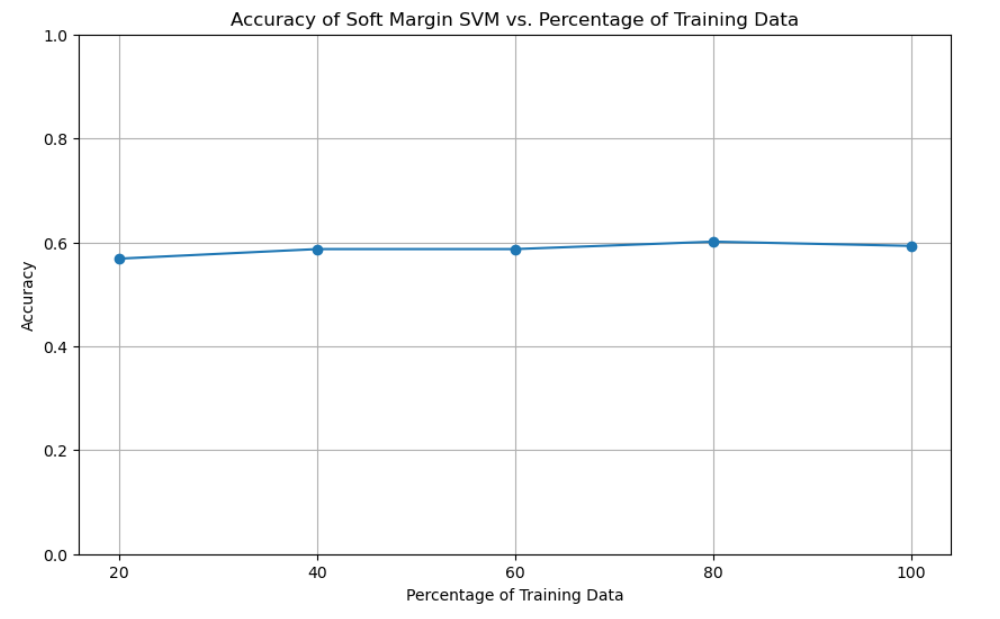
\includegraphics[width=0.7\linewidth]{template/Plots/unicode_part1.png}
    \caption{Accuracy plot for unicode representation}
    \label{fig:1}
\end{figure}

We then went on try one-hot encoding of the emoticons. The code snippet of the same is: 

\begin{lstlisting}[language=Python]
unique_emojis = set()
for i in train_emoticon_X:
    unique_emojis.update(list(i))
unique_emojis = list(unique_emojis)

#All the unique emojis collected from each string of emoticons. Next part is creating emoji-to-index dictionary

emoji_to_index = {emoji: idx for idx, emoji in enumerate(unique_emojis)}

# One-hot encoding function for a single emoji
def one_hot(emoji):
    encoding = np.zeros(len(unique_emojis), dtype=int)
    if emoji in emoji_to_index:
        index = emoji_to_index[emoji]
        encoding[index] = 1
    return encoding

# We finally need one_hot encoding function for a sequence of 13 emojis
def one_hot_encode_and_concatenate(emoji_sequence):
    concatenated_vector = np.zeros(13 * len(unique_emojis), dtype=int) 
    # 13 one-hot vectors concatenated
    for idx, emoji in enumerate(emoji_sequence[:13]):
        one_hot_vector = one_hot(emoji)  # One-hot encode each emoji
        concatenated_vector[idx * len(unique_emojis):(idx + 1) * len(unique_emojis)] = one_hot_vector  # Concatenate
    return concatenated_vector
    
train_X = input_emoticon_X.apply(one_hot_encode_and_concatenate)

# Convert the result into a 2D numpy array for training (batch_size x 13 * num_unique_emojis)
train_X = np.stack(train_X)

valid_X = valid_emoticon_X.apply(one_hot_encode_and_concatenate)
valid_X = np.stack(valid_X)

\end{lstlisting}

We have calculated the number of unique emojis as $214$ for the training dataset (as well as test dataset) so the size of individual input is $214*13 = 2782$ (this will be useful later when we calculate the number of trainable parameters in task 2). On this encoding, we tried different models like DTs, Logistic Regression, SVMs and it lead us to the following accuracy plot:

\begin{figure}[h!]
    \centering
    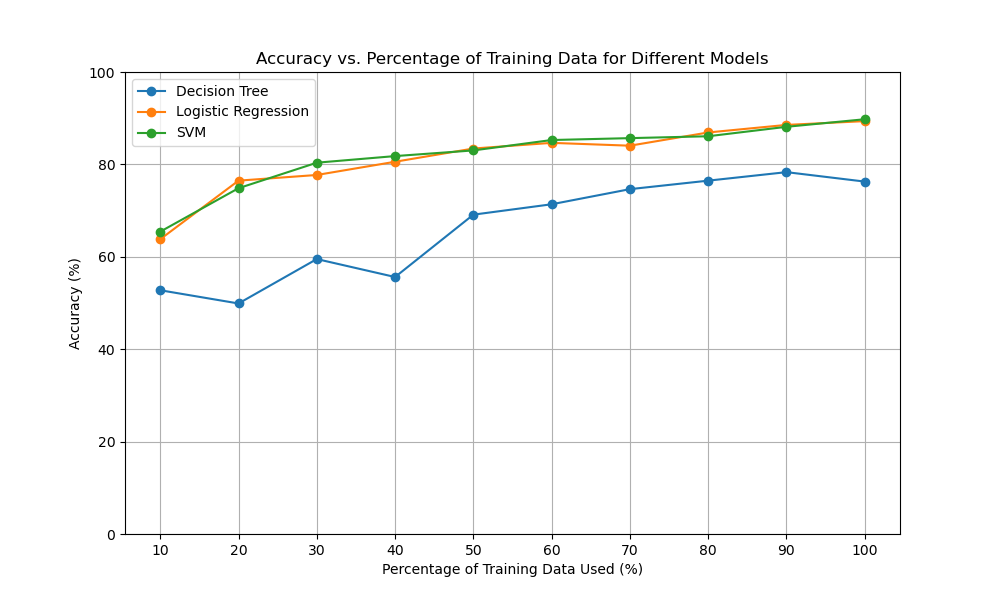
\includegraphics[width=1\textwidth]{template/Plots/one-hot.png}
    \caption{Plot of accuracy vs percentage of training data used}
    \label{fig:2}
\end{figure}
This was the maximum we could achieve using one-hot encoding. As it was allowed to use pre-trained deep learning model as feature extractor, we decided to learn\footnote{\href{https://huggingface.co/sentence-transformers}{Hugging face's}documentation was of big help} and use them directly for our feature transformation to improve our accuracy! That didn't go quite well (maybe we didn't use suitable neural-based encoding, who knows): 
\begin{lstlisting}[language=Python]
    models_to_test = [
    'all-MiniLM-L6-v2',
    'distilbert-base-nli-stsb-mean-tokens',
    'roberta-base-nli-stsb-mean-tokens',
    'bert-base-nli-mean-tokens'
    ]
\end{lstlisting}

Encoding the dataset emoticons using the first one in the above models gave us the graph given below:
\begin{figure}[h!]
    \centering
    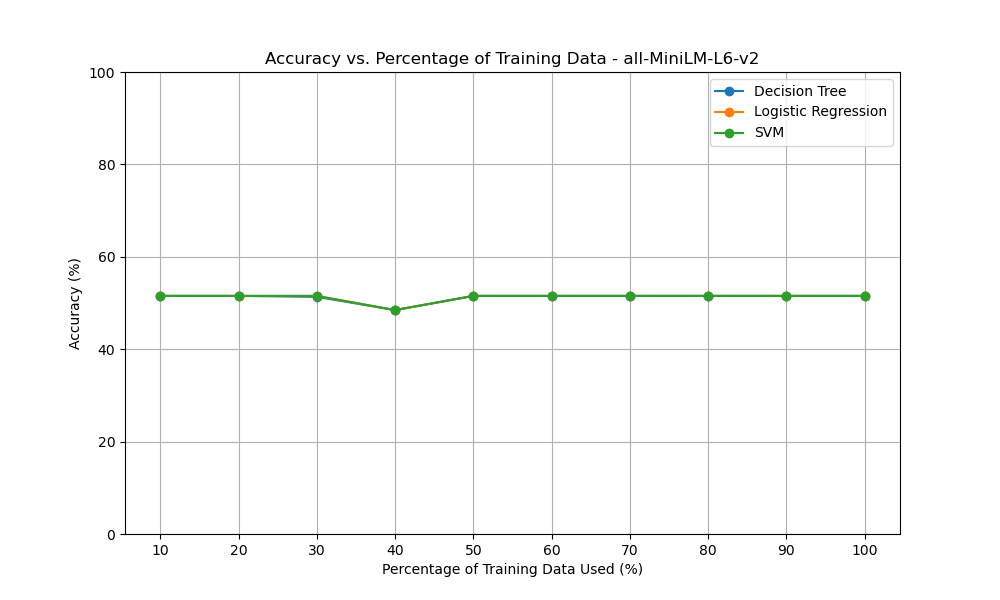
\includegraphics[width=0.4\textwidth]{template/Plots/all-mini.png}
    \caption{Using all-MiniLM-L6-v2 sentence transformer}
    \label{fig:3}
\end{figure}


We also tried KNN and LwP based on these transformers but their accuracy also wasn't good anyway. This wasn't nearly enough. We then tried DTs, Logistic Regression, SVM, etc for the distilbert-base-nli-stsb-mean-tokens neural-based transformer and other ones as well but they didn't yield any plots with decent accuracy. We realized later that the extracted features from transformers face lot of collisions i.e. for two different sequences of emoticons we get the same encoding, which results in bad accuracy. We also tried RNN and CNN for feature extraction but they also gave nearly 50\% accuracy 


% \begin{figure}[h!]
%     \centering
%     \includegraphics[width=0.8\textwidth]{plot.png}
%     \caption{Sample Plot Generated in Python}
%     \label{fig:sample_plot}
% \end{figure}



% \begin{figure}
%     \centering
%     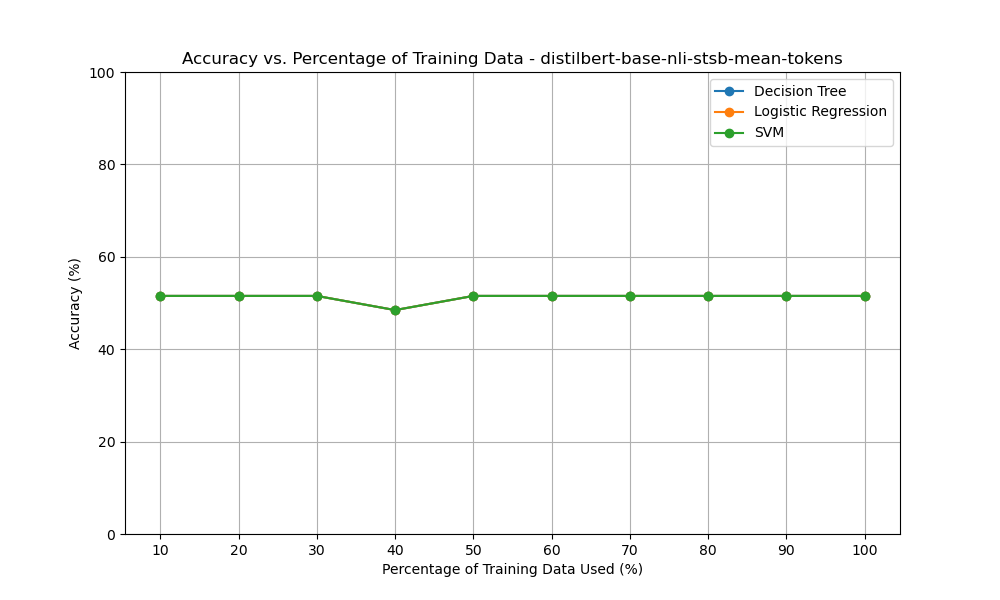
\includegraphics[width=0.8\linewidth]{template/Plots/distilbert.png}
%     \caption{Using distibert-base-nli-stsb-mean-tokens}
%     \label{fig:enter-label}
% \end{figure}
\subsection{Deep Features Dataset}
For this dataset, we decided to use Averaging (which was mentioned in the question itself), Max Pooling, Concatenation, and a neural based feature extractor (CNN). For each of these encodings, we tried DTs, Logistic Regression, SVM and other models.

\begin{lstlisting}[language=Python]
# 1. Averaging Embeddings
train_feat_X_avg = np.mean(train_feat_X, axis=1)
valid_feat_X_avg = np.mean(valid_feat_X, axis=1)
accuracies_avg = evaluate_decision_tree(train_feat_X_avg, valid_feat_X_avg)

# 2. Concatenation of Embeddings
train_feat_X_concat = train_feat_X.reshape(train_feat_X.shape[0], -1)
valid_feat_X_concat = valid_feat_X.reshape(valid_feat_X.shape[0], -1)
accuracies_concat = evaluate_decision_tree(train_feat_X_concat, valid_feat_X_concat)

# 3. MaxPooling of Embeddings
train_feat_X_maxpool = np.max(train_feat_X, axis=1)
valid_feat_X_maxpool = np.max(valid_feat_X, axis=1)
accuracies_maxpool = evaluate_decision_tree(train_feat_X_maxpool, valid_feat_X_maxpool)
# 4. Standard CNN-based Embedding Extraction
def build_cnn_model():
    model = models.Sequential()
    model.add(layers.Conv1D(filters=32, kernel_size=3, activation='relu', input_shape=(13, 768)))
    model.add(layers.MaxPooling1D(pool_size=2))
    model.add(layers.Conv1D(filters=64, kernel_size=3, activation='relu'))
    model.add(layers.MaxPooling1D(pool_size=2))
    model.add(layers.Flatten())
    return model

cnn_model = build_cnn_model()
cnn_model.compile(optimizer='adam', loss='binary_crossentropy', metrics=['accuracy'])

# Get CNN features
train_feat_cnn = cnn_model.predict(train_feat_X)
valid_feat_cnn = cnn_model.predict(valid_feat_X)
accuracies_cnn = evaluate_decision_tree(train_feat_cnn, valid_feat_cnn, "CNN")
\end{lstlisting}
As the number of trainable parameters in CNN exceed the limit, we have not included it in the final code. 
\subsubsection{Decision Tree}
We started off with the decision tree which gave us below plot:

\begin{figure}[htbp]
    \centering
    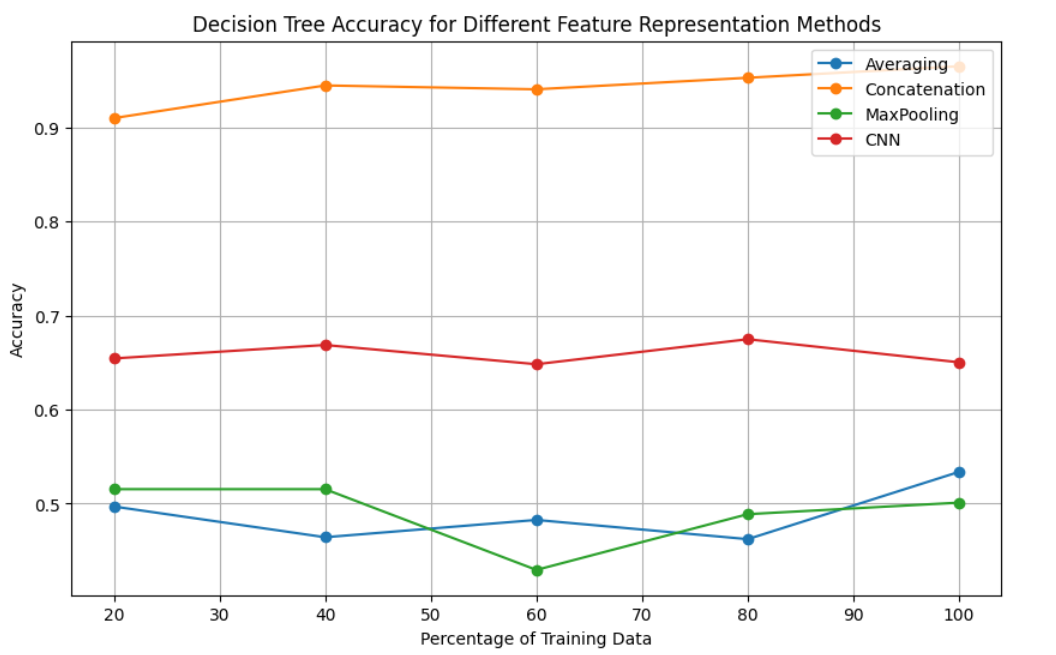
\includegraphics[width=0.4\linewidth]{template/Plots/DT_part2.png}
    \caption{Decision Tree accuracy based on different feature extraction methods.}
    \label{fig:4}
\end{figure}
\subsubsection{Logistic Regression}
We then went on to try Logistic Regression which gave us the following plot: 
\begin{figure}[htbp]
    \centering
    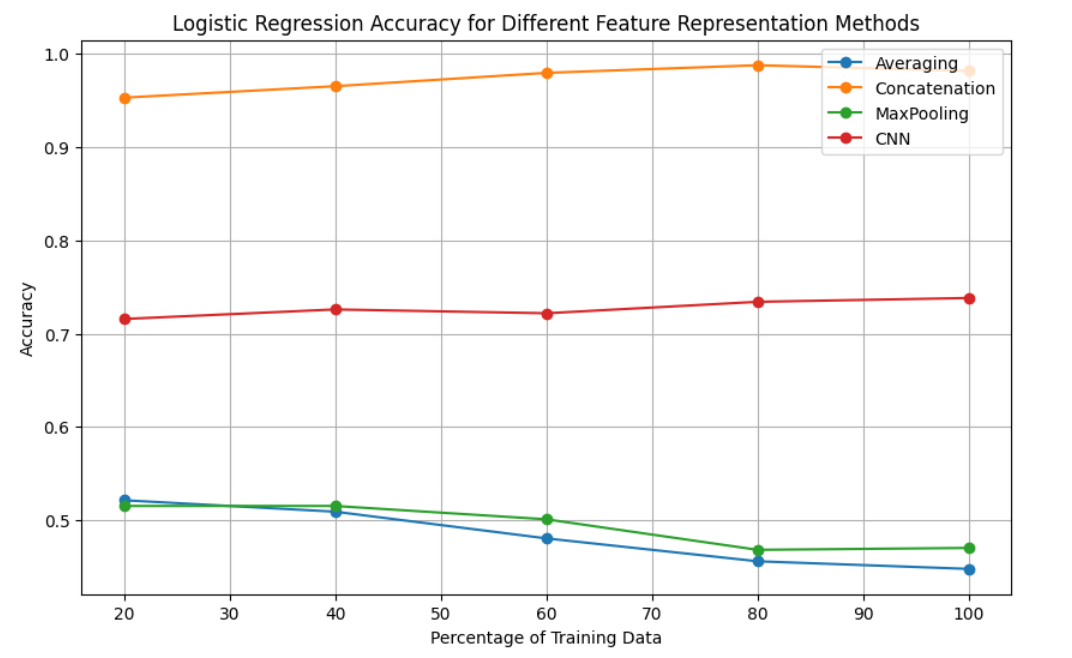
\includegraphics[width=0.5\linewidth]{template/Plots/lr_part2.png}
    \caption{Logistic Regression accuracy based on different feature extraction methods.}
    \label{fig:5}
\end{figure}
\subsubsection{Support Vector Machine}
The plot for support vector machine is given below:
% \subsection{Subsection (if any) Name}
\begin{figure}[htbp]
    \centering
    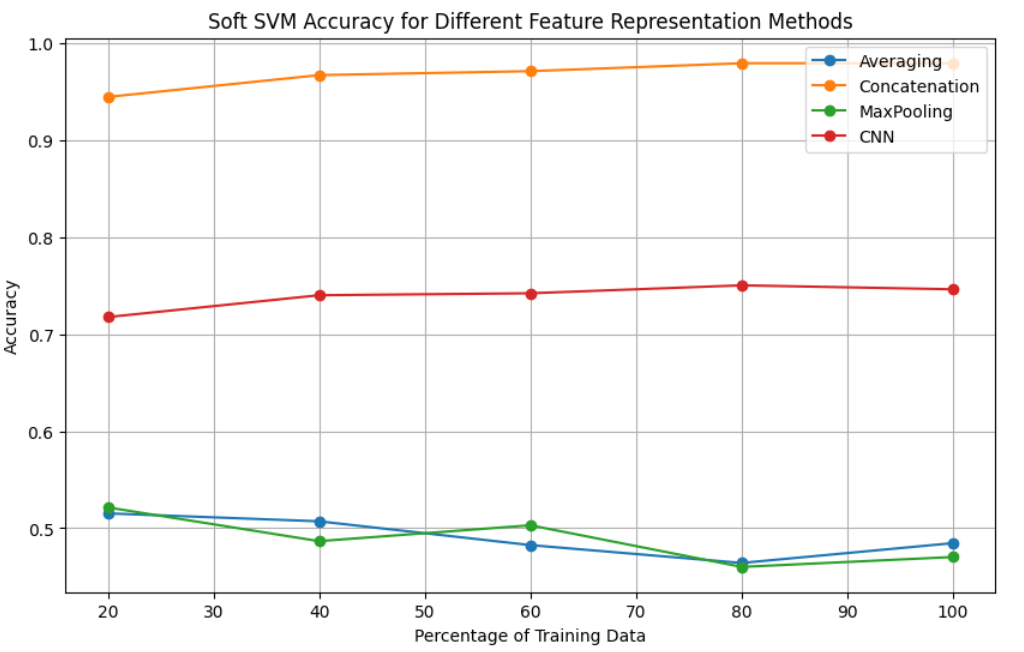
\includegraphics[width=0.5\linewidth]{template/Plots/softsvm_part2.png}
    \caption{Soft Margin SVM accuracy based on different feature extraction methods.}
    \label{fig:6}
\end{figure}
\subsubsection{Final Code}
We observe that concatenation is giving us maximum accuracy across all the feature extraction methods. We have combined the plots of all the models for concatenation below:

\begin{figure}[htbp]
    \centering
    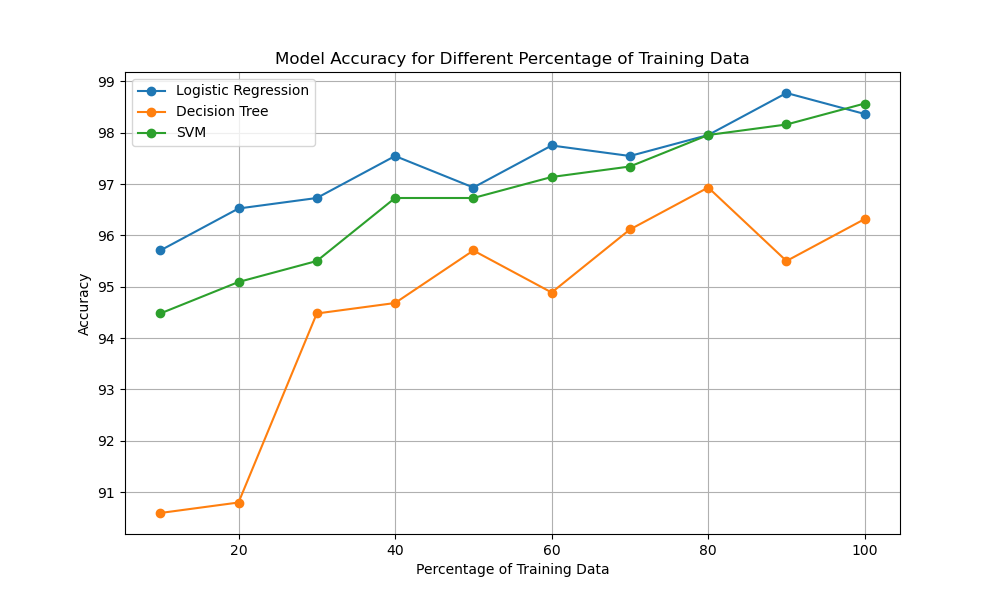
\includegraphics[width=0.8\linewidth]{template/Plots/task1_part3_fig.png}
    \caption{Accuracies of different models for concatenation}
    \label{fig:7}
\end{figure}
It can be seen from the above figure that the logistic regression is performing relatively better than the other models. The code snippet for logistic regression is given below:

\begin{lstlisting}[language=Python]
percentages = [0.1, 0.2, 0.3, 0.4, 0.5, 0.6, 0.7, 0.8, 0.9, 1.0]

def evaluate_LR(train_feat_X_method, valid_feat_X_method, method_name):
    accuracies = []
    for percentage in percentages:
        n_samples = int(len(train_feat_X_method) * percentage)
        x_train_subset = train_feat_X_method[:n_samples]
        y_train_subset = train_feat_Y[:n_samples]
        LR_classifier = LogisticRegression(random_state=42)
        LR_classifier.fit(x_train_subset, y_train_subset)

        # Predict on the validation set
        y_pred = LR_classifier.predict(valid_feat_X_method)

        # Calculate accuracy
        accuracy = accuracy_score(valid_feat_Y, y_pred)
        accuracies.append(accuracy)
    
    return accuracies
# Concatenation of Embeddings
train_feat_X_concat = train_feat_X.reshape(train_feat_X.shape[0], -1)
valid_feat_X_concat = valid_feat_X.reshape(valid_feat_X.shape[0], -1)
accuracies_concat = evaluate_LR(train_feat_X_concat, valid_feat_X_concat, "Concatenation")
    
\end{lstlisting}
The corresponding plot is shown below: 
\begin{figure}[htbp]
    \centering
    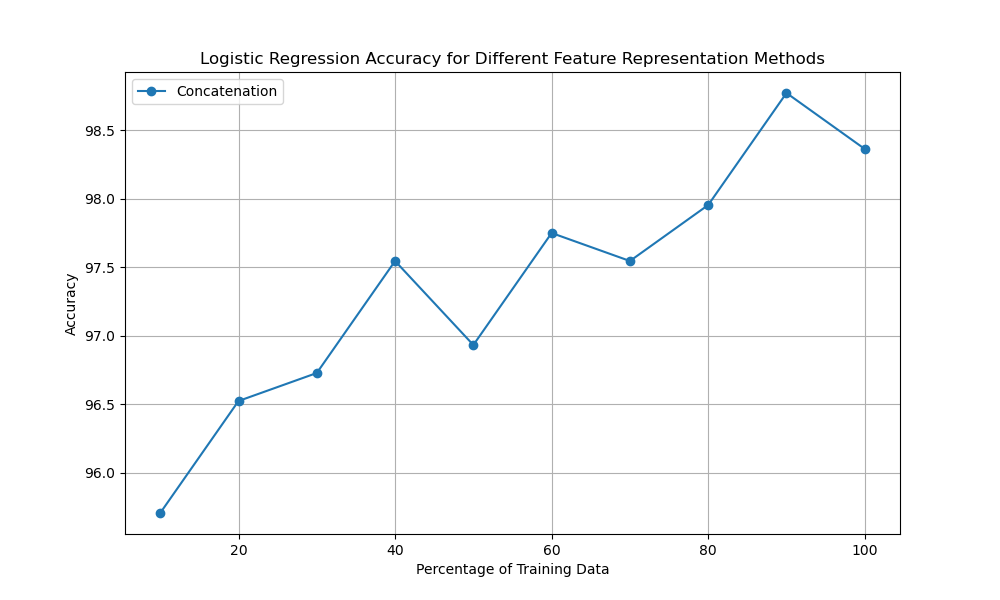
\includegraphics[width=1\linewidth]{template/Plots/lr_final.png}
    \caption{Logistic Regression accuracy with concatenation feature extractor.}
    \label{fig:8}
\end{figure}
\subsection{Text Sequence Dataset} 
We decided to first convert the string into a sequence of integers, rather we could have directly passed string as an input parameter in the model but these models generally work with numerical data inputs, so changing it into a sequence of integers is a better choice. 

\begin{lstlisting}[language=Python]
# Preprocessing: Convert input strings to sequences of integers
max_length = 50
train_seq_X = [[int(digit) for digit in seq] for seq in train_seq_X]
valid_seq_X = [[int(digit) for digit in seq] for seq in valid_seq_X] 
# Preprocess validation data
train_seq_X = np.array(train_seq_X)
valid_seq_X = np.array(valid_seq_X)

#Convert it into numpy array
train_seq_Y = np.array(train_seq_Y)
valid_seq_Y = np.array(valid_seq_Y)

# Define CNN Model architecture with reduced parameters
def build_cnn_model(input_shape):
    model = Sequential()
    model.add(Embedding(input_dim=10, output_dim=16, input_length=input_shape[1]))  # Reduced embedding dimension
    model.add(Conv1D(16, kernel_size=3, activation='relu'))  # Reduced number of filters
    model.add(MaxPooling1D(pool_size=2))
    model.add(Flatten())
    model.add(Dense(16, activation='relu'))  # Reduced dense layer size
    model.add(Dropout(0.3))
    model.add(Dense(1, activation='sigmoid'))  # For binary classification
    model.compile(optimizer='adam', loss='binary_crossentropy', metrics=['accuracy'])
    return model

# Function to train models and record validation accuracy
def train_model_on_subsets(model_func, model_type, X_train, y_train, X_val, y_val):
    percentages = [0.2, 0.4, 0.6, 0.8, 1.0]
    accuracies = []
    
    for p in percentages:
        subset_size = int(len(X_train) * p)
        X_train_subset = X_train[:subset_size]
        y_train_subset = y_train[:subset_size]

        if model_type == "CNN":
            # Build and train the CNN model
            model = model_func(X_train_subset.shape)
            model.fit(X_train_subset, y_train_subset, epochs=10, batch_size=64, verbose=0)
            y_val_pred = (model.predict(X_val) > 0.5).astype("int32")
            val_accuracy = accuracy_score(y_val, y_val_pred)
        else:
            # Train traditional machine learning models
            model = model_func()
            model.fit(X_train_subset, y_train_subset)
            y_val_pred = model.predict(X_val)
            val_accuracy = accuracy_score(y_val, y_val_pred)

        accuracies.append(val_accuracy)

    return percentages, accuracies

# Different models we have used
models = {
    "Logistic Regression": lambda: LogisticRegression(max_iter=1000),
    "kNN": lambda: KNeighborsClassifier(n_neighbors=5),
    "Decision Tree": lambda: DecisionTreeClassifier(),
    "Soft Margin SVM": lambda: SVC(kernel='linear', C=1),
    "CNN": build_cnn_model
}
\end{lstlisting}
Initially, the number of trainable parameters exceeded the 10,000 trainable parameters constraint. We then reduced the number of filters and dense layer size to satisfy the constraint.
\begin{figure}
    \centering
    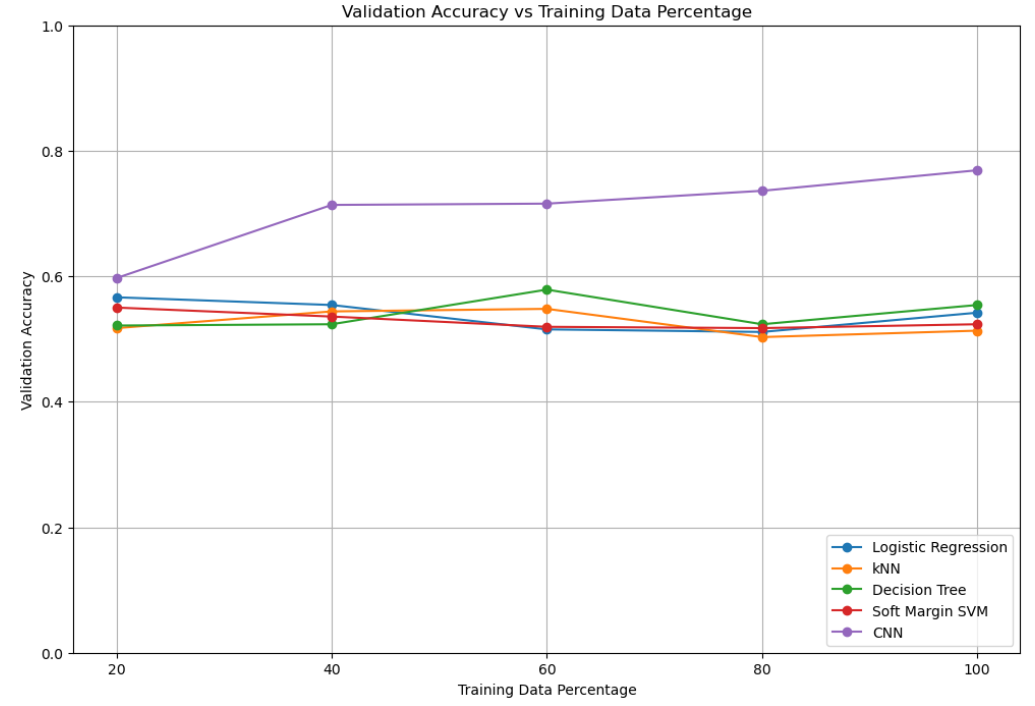
\includegraphics[width=0.8\linewidth]{template/Plots/final_part3.png}
    \caption{Final Plot of accuracies for different models.}
    \label{fig:9}
\end{figure}

\subsubsection{Further Exploration}
We decided to use neural-based feature extractors with the hope of achieving better accuracy. 
\begin{lstlisting}[language=Python]
def build_embedding_model():
    model = tf.keras.Sequential()
    model.add(Embedding(input_dim=vocab_size, output_dim=embedding_dim, input_length=max_length))
    model.add(GlobalAveragePooling1D())
    return model

def build_cnn_model():
    model = tf.keras.Sequential()
    model.add(Embedding(input_dim=vocab_size, output_dim=embedding_dim, input_length=max_length))
    model.add(Conv1D(filters=32, kernel_size=3, activation='relu'))
    model.add(GlobalAveragePooling1D())
    return model

def build_rnn_model():
    model = tf.keras.Sequential()
    model.add(Embedding(input_dim=vocab_size, output_dim=embedding_dim, input_length=max_length))
    model.add(SimpleRNN(64))
    return model

def build_lstm_model():
    model = tf.keras.Sequential()
    model.add(Embedding(input_dim=vocab_size, output_dim=embedding_dim, input_length=max_length))
    model.add(LSTM(64))
    return model
\end{lstlisting}
For the above feature extractors, we got the following accuracy plot for different models:

\textbf{1.3.1.1.\hspace{0.3cm}Decision Tree}
\begin{figure}[htbp]
    \centering
    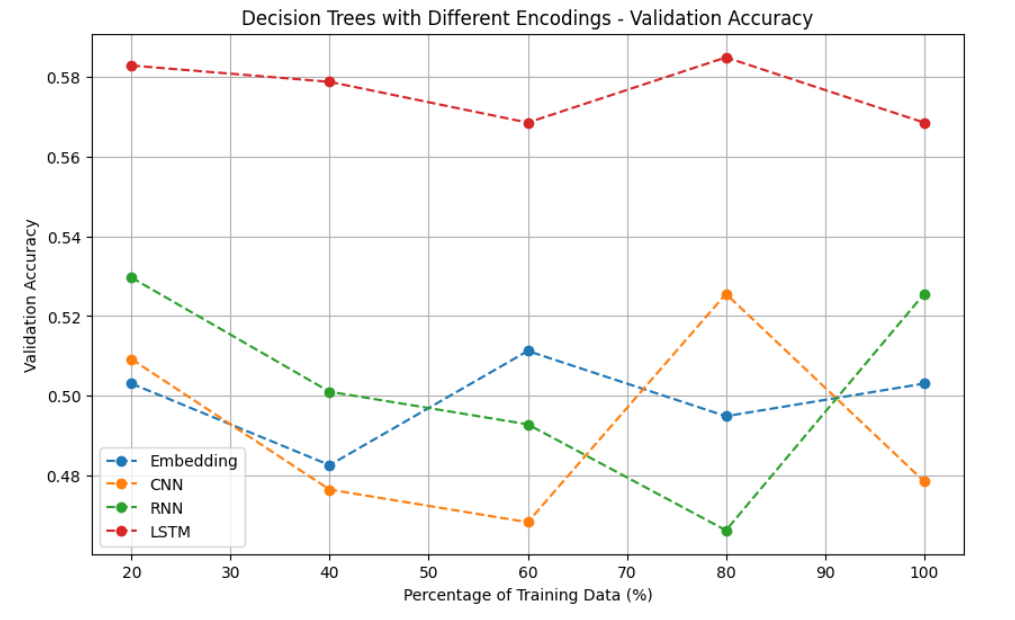
\includegraphics[width=0.3\linewidth]{template/Plots/dt_part3.png}
    \caption{Decision Tree accuracy for different neural network-based feature extractors.}
    \label{fig:10}
\end{figure}

\textbf{1.3.1.2.\hspace{0.3cm}Logistic Regression}
\begin{figure}[htbp]
    \centering
    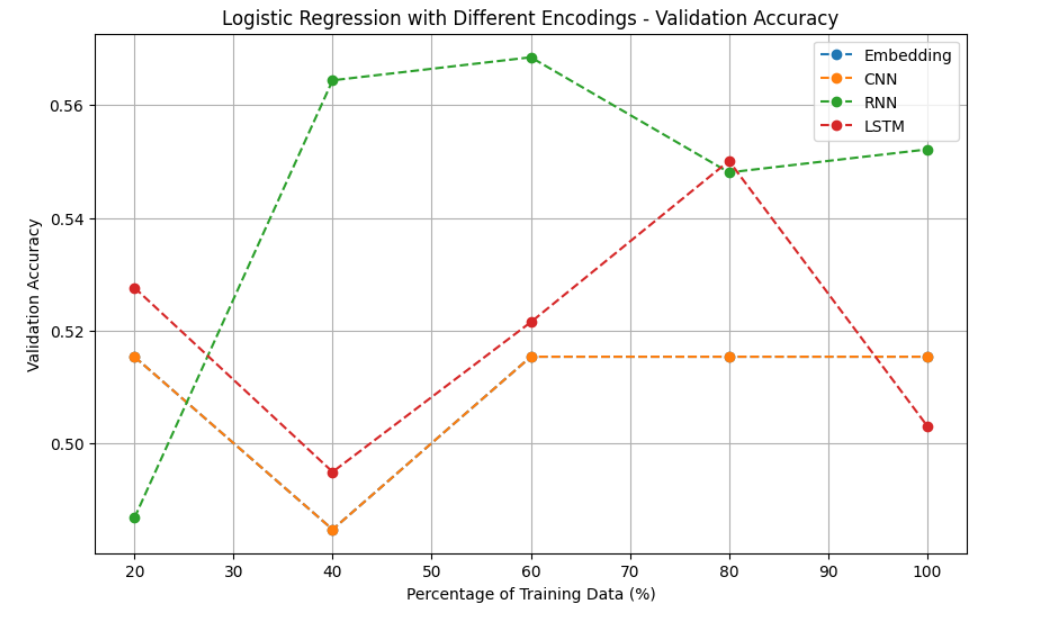
\includegraphics[width=0.5\linewidth]{template/Plots/lr_part3.png}
    \caption{Logistic Regression accuracy for different neural network-based feature extractors.}
    \label{fig:11}
\end{figure}

\textbf{1.3.1.3.\hspace{0.3cm}Support Vector Machine}
\begin{figure}[htbp]
    \centering
    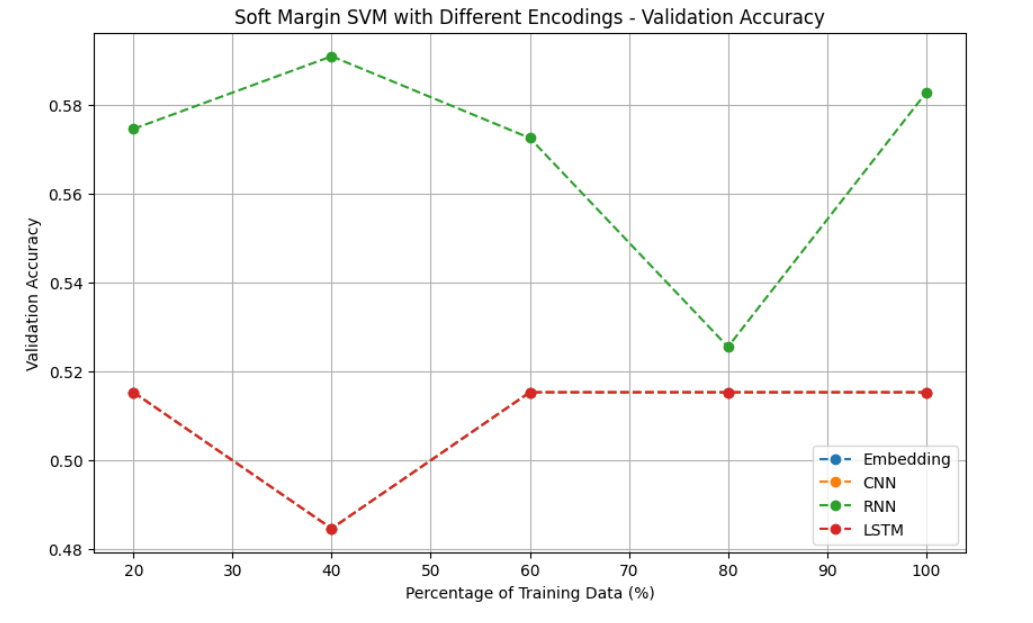
\includegraphics[width=0.5\linewidth]{template/Plots/svm_part3.png}
    \caption{SVM accuracy for different neural network-based feature extractors.}
    \label{fig:12}
\end{figure}
% \subsubsection{.1 Decision Tree}

\section{Task 2}
As we can see that in second part of task 1, we have achieved an accuracy of approximately $98.5\%$, so when we combine all the datasets from all the parts, we hope to get better accuracy than this. We tried to concatenate all the dataset inputs into one. The input size of first datset is $2782$, second dataset is $9984$, third dataset is $50$ which in total exceeds our constraint of trainable parameters ($1000$). So we have used PCA to reduce the dimensionality of the second dataset to $7000$. 
\begin{figure}[htbp]
    \centering
    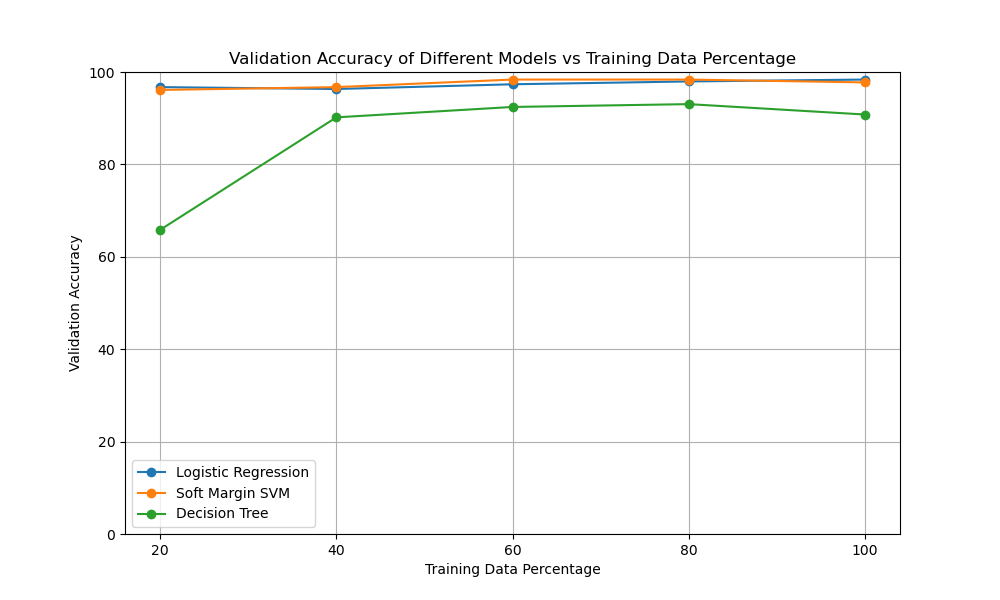
\includegraphics[width=0.6\linewidth]{template/Plots/task2_combined.png}
    \caption{Accuracy plot for different models when the dimensionality of second dataset is $7000$}
    \label{fig:13}
\end{figure}

The code snippet for the above plot is: 

\begin{lstlisting}[language=Python]
# Prepare the third dataset: digit encoding
max_length = 50
train_seq_X_encoded = [[int(digit) for digit in seq] for seq in train_seq_X]
train_seq_X_encoded = np.array(train_seq_X_encoded)

valid_seq_X_encoded = [[int(digit) for digit in seq] for seq in valid_seq_X]
valid_seq_X_encoded = np.array(valid_seq_X_encoded)

# Feature Transformation
# One-Hot Encoding for Emoticons
encoder = OneHotEncoder(sparse_output=False, handle_unknown = 'ignore')
train_emoticon_X_encoded = encoder.fit_transform(np.array(train_emoticon_X).reshape(-1, 1))
valid_emoticon_X_encoded = encoder.transform(np.array(valid_emoticon_X).reshape(-1, 1))


# Flatten the feature matrix
train_feat_X_reshaped = train_feat_X.reshape(train_feat_X.shape[0], -1) 

# Flatten the feature matrix
valid_feat_X_reshaped = valid_feat_X.reshape(valid_feat_X.shape[0], -1)  

# Apply PCA to reduce deep features to 7,000 features
pca = PCA(n_components=7000)  # Adjust number of components as needed
train_feat_X_reduced = pca.fit_transform(train_feat_X_reshaped)
valid_feat_X_reduced = pca.transform(valid_feat_X_reshaped)

# Concatenate Deep Features (after PCA) with One-Hot Encoded Features
combined_train_features = np.concatenate((train_feat_X_reduced, train_emoticon_X_encoded), axis=1)
combined_valid_features = np.concatenate((valid_feat_X_reduced, valid_emoticon_X_encoded), axis=1)

# Concatenate the Combined Features with Digit Encoded Features
final_train_features = np.concatenate((combined_train_features, train_seq_X_encoded), axis=1)
final_valid_features = np.concatenate((combined_valid_features, valid_seq_X_encoded), axis=1)


final_train_labels = train_seq_Y
final_valid_labels = valid_seq_Y

# Define models
models = {
    "Logistic Regression": LogisticRegression(max_iter=1000),
    "Soft Margin SVM": SVC(kernel='linear', C=1),
    "Decision Tree": DecisionTreeClassifier()
}

# Store results for plotting
percentages = [0.2, 0.4, 0.6, 0.8, 1.0]  # Training percentages
results = {model_name: [] for model_name in models.keys()}  # Initialize results

# Train on subsets of the training data
for p in percentages:
    subset_size = int(len(final_train_features) * p)
    X_train_subset = final_train_features[:subset_size]
    y_train_subset = final_train_labels[:subset_size]

    for model_name, model in models.items():
        model.fit(X_train_subset, y_train_subset)
        
        # Evaluate on the validation set
        y_val_pred = model.predict(final_valid_features)  # Use the validation features
        val_accuracy = accuracy_score(final_valid_labels, y_val_pred)

        results[model_name].append(val_accuracy*100)

# Plotting the results
plt.figure(figsize=(10, 6))
for model_name, accuracies in results.items():
    plt.plot([p * 100 for p in percentages], accuracies, marker='o', label=model_name)

plt.title("Validation Accuracy of Different Models vs Training Data Percentage")
plt.xlabel("Training Data Percentage")
plt.ylabel("Validation Accuracy")
plt.xticks([20, 40, 60, 80, 100])
plt.ylim(0, 100)  # Set y-axis limits for clarity
plt.grid()
plt.legend()
plt.show()
    
\end{lstlisting}
This PCA uses the entire dataset to extract features and reduce dimensionality of the deep features dataset, we have found the accuracy of logistic regression to be the highest across all the $3$ models mentioned above, which is $98.16\%$ which was already not a marginal improvement over our original accuracy for the second dataset, so it can be inferred that on applying PCA on incremental fractions of data will definitely give even lesser accuracy.







We have tried above approaches but we coudn't get any marginal improvement over accuracy obtained in deep features dataset. The second dataset seems to be the most accurate representation of the distribution on which the all the datasets are based. Therefore, we will use the deep features dataset to make predictions on test data.

\bibliography{cs698x_project}
\bibliographystyle{plain}
\begin{itemize}
    \item Used the \href{https://scikit-learn.org/stable/supervised_learning.html}{sk-learn} documentation for classification.
    \item Read about \href{https://huggingface.co/models?library=sentence-transformers&sort=downloads}{Sentence Transformers} from Hugging Face.
    \item Learnt about tensor flow from its \href{https://www.tensorflow.org/tutorials}{documentation}.
    \item Took help of chat-gpt in debugging codes. 
\end{itemize}
\end{document}
